\documentclass[10pt,twocolumn]{confpaper}

%%%%%%%%%%%%%%%%%%%%  INCLUDES  %%%%%%%%%%%%%%%%%%%%%%%%%%
\usepackage{pifont}
\usepackage{algorithm}
\usepackage{algorithmic}
\usepackage{url}
\usepackage{breakurl} 
%%%%%%%%%%%%%%%%%%%%  LOCALS  %%%%%%%%%%%%%%%%%%%%%%%%%%%%

\def\UrlBreaks{\do\/\do-}
\newcommand{\system}{{OCDN}}
\def\checkmark{\tikz\fill[scale=0.4](0,.35) -- (.25,0) -- (1,.7) -- (.25,.15) -- cycle;}
\graphicspath{ {./figures/} }
\newcommand{\annie}[1]{\emph{\color{blue}(#1)}}


%%%%%%%%%%%%%%%%%%%%  TITLE/AUTHORS  %%%%%%%%%%%%%%%%%%%%%

\date{}
\title{\LARGE{\bf OCDN: Oblivious Content Distribution Networks}}
\author{
\aufnt{} \\
\affaddr{}
}

%%%%%%%%%%%%%%%%%%%%  START OF DOCUMENT  %%%%%%%%%%%%%%%%%

\begin{document}

\maketitle

%\AcmCopyright
%\ToAppear

\begin{sloppypar}




\begin{abstract}  
As publishers increasingly use Content Distribution Networks
(CDNs) to distribute content across geographically diverse networks of
proxies, CDNs themselves are becoming unwitting targets of requests for both
access to user data and content takedown. From copyright infringement to
moderation of online speech, CDNs have found themselves at the forefront of a
many recent legal quandaries. At the heart of the tension, however, is the fact
that CDNs have rich information both about the content they are serving and the
users who are requesting that content. 
This paper offers a technical contribution that relevant to this ongoing tension
with design of an Oblivious CDN (OCDN), a CDN that is both compatible with the existing
Web ecosystem of publishers and
clients and hides from the CDN both the content it is serving and the users
who are requesting that content. \system{} is compatible with the way that publishers
currently host content on CDNs. Publishers can use multiple CDNs to publish content
via \system{}; clients retrieve content through a peer-to-peer anonymizing network
of proxies.
Our prototype implementation and
evaluation of \system{} show that the system can obfuscate both content and clients
from the CDN operator while still delivering content with good performance.
\end{abstract}

\ifthenelse{\equal{\onlyAbstract}{no}}{% !onlyAbstract


\section{Introduction}
\label{sec:intro}

As the structure of the Internet continues to evolve, the ways in which 
data and communications are governed also continue to change.  Data can 
be generated by a citizen of one country, stored in a different country 
on servers belonging to a company headquartered in yet another country.  
Additionally, data can flow from one country to another by transiting a 
variety of other countries.  As the Internet is a global system spanning 
many nation states, this raises the question of how these data are 
governed, and under what circumstances are governments are allowed to access what
data.

%The policies and behavior of different nation states provide different 
%treatment of data.  These differences occur in policies regarding net 
%neutrality, copyright enforcement, data privacy protection, etc. For example, 
%some countries, such as the United States, Canada, parts of South America, parts 
%of Europe, India, Japan, and South Korea have either laws or regulations for 
%protecting net neutrality, where as other countries, such as Russia, China, and Myanmar, 
%have no net neutrality laws or regulations \cite{net_neutrality}.  Similarly, different 
%jurisdictions have different policies and enforcement of copyright infringement; both 
%the United States and China have signed onto major international copyright treaties, but 
%China has no notion of ``fair use,'' meaning someone can reproduce a copyrighted work 
%without permission if it falls under a range of excepted categories, while the United 
%States does \cite{copyright}.  We can see that as data is produced, distributed, and stored 
%around the world --- in large part due to the Internet --- we face the question of which 
%jurisdiction, and subsequently which policies, does it fall under.

A clear example of such a scenario where there are cross-jurisdictional issues is that of 
a Content Delivery Network (CDN).  A CDN consists of a set of cache nodes, which replicate 
and distribute content produced by other entities.  In our example, Alice has a blog and lives in Russia.  
She is a customer of a CDN, which replicates her 
content on a cache node in France.  The CDN is headquartered 
in the United States and operates cache nodes around the world.  There are two separate questions that should 
be addressed: 1) What type of information could an overreaching government demand? 2) Which government 
(if any) should legally be allowed to demand the data?  For the first question, some information that may be 
demanded of the CDN is the identity of a specific content owner or a list of which clients are accessing which content. 
In response to the second question, there is currently no clear answer to which jurisdiction has legal 
right to the CDN's data.  The United States could argue for the data because the CDN is headquartered 
there; Russia could argue for the data because the content publisher resides there; France could argue for the data 
because the data is located there. 

The stakeholders in this 
example are the content owner, the CDN, and the Internet users --- and each of these entities differ in what 
they have at stake.  Alice may be punished for publishing content that is politically controversial; the CDN 
may be held liable for controversial information (or copyright infringements); the Internet users' 
privacy could be leaked.  Each stakeholder should be interested (and possibly worried) about the 
consequences of overreaching government access.  In fact, we have recently seen that Cloudflare, a popular 
CDN, has been secretly required to hand over data to the FBI~\cite{cloudflare_gag}.  Similarly, leaked 
NSA documents showed that the government agency ``collected information `by exploiting inherent weaknesses 
in Facebook's security model' through its use of the popular Akamai content delivery network''~\cite{}.

In this work, we focus on the privacy implications of cross-border data flows and data 
storage, and how technology can be designed to protect citizens' data, regardless of the 
jurisdiction in which the client, data, or service resides.  In light of 
the Snowden revelations, many countries have taken 
measures to avoid United States surveillance on their citizens' Internet traffic; some of 
the ways some countries are avoiding known surveillance states include: controlling the route 
that Internet traffic takes by deploying underwater cables that avoid surveillance states~\cite{brazil}; 
requiring their citizens' data to be stored locally, so as to prevent their citizens' data from 
being stored in a country that conducts surveillance~\cite{russia}; controlling Internet paths by building 
IXPs; halting the use of technology designed and developed in surveillance states.  While some of these 
solutions are technical, many are political, and in most cases solutions come from court decisions, not 
technology.

While policy and regulation are being created and challenged, technologists have a role 
in this area too.  Technology and systems can be developed to facilitate data privacy in the 
face of an overreaching government or conflicting jurisdictional policies.  Not only can 
these systems protect Internet users' privacy, but they can also provide protections 
for content creators and content distributors (regardless of their geographic location).  

In this paper, we provide background on some of the jurisdictional differences 
on both data in motion and data at rest, discuss historical and current laws and cases of 
government access to data (in motion and at rest), as well as put these cases into the context 
of technology development. We also highlight current systems that aim to protect data privacy from nation 
state adversaries, and discuss how they stop short of circumventing nation state surveillance.  Lastly, we
 point out the gaps in this technology landscape, and 
subsequently call for future work.

These systems and techniques should be applied to two separate types of data: 1) data in 
motion and 2) data at rest.  We differentiate between these two types of data for a number of reasons.  
First, there are different policies and regulations applicable to the two types of data.  Second, 
they have different characteristics, which lead to different technological requirements to preserve 
privacy from nation-state surveillance, especially considering this surveillance can come from  
wiretapping or serving a subpoena.

The rest of the paper is organized as follows.  We discuss data in motion in more depth in Section \ref{sec:motion}, where we highlight 
historical cases, current issues, and how technology can provide protection in this domain.  We also highlight and compare
systems proposed in the literature that protect the privacy of data in motion. Section \ref{sec:rest} 
points out the important cases in regards to data at rest, as well as how technology should be designed 
differently for this type of data in comparison to data in motion.  We discuss related work in Section \ref{sec:related} and 
conclude in Section \ref{sec:conclusion}.

\section{Background}
\label{sec:background}

We now outline how a CDN typically operates, what information it
has access to by virtue of running a CDN, and some of the ongoing legal battles
surrounding CDNs.

\subsection{Content Distribution Networks}
CDNs provide content caching as a service to content publishers.  A 
content publisher may wish to use a CDN provider for a number of reasons:

\begin{itemize}
\item CDNs cache content in geographically distributed locations, which allows for localized 
data centers, faster download speeds, and reduces the load on the content publisher's server.
\item CDNs typically provide usage analytics, which can help a content publisher get a better 
understanding of usage as compared to the publisher's understanding without a CDN.
\item CDNs provide a high capacity infrastructure, and therefore provide higher availability, 
lower network latency, and lower packet loss.  
\item CDNs' data centers have high bandwidth, which allows them to handle and mitigate DDoS attacks better 
than the content publisher's server.
\end{itemize}

CDN providers usually have a large number of edge servers on which content is cached; for example, 
Akamai has more than 216,000 servers in over 120 countries around the world~\cite{akamai_facts}.  
Having more edge servers in more locations increases the probability that a cache is geographically 
close to a client, and could reduce the end-to-end latency, as well as the likelihood of some kinds of 
attacks, such as BGP (Border Gateway Protocol) hijacking.  This is evident when a client requests a web page; the closest 
edge server to the client that contains the content is identified and the content is served from that 
edge server.  Most often, this edge server is geographically closer to the client than the content publisher's 
server, thus increasing the speed in which the client receives the content. If the requested page's content is 
not in one of the CDN's caches, then the request is forwarded to the content publisher's server, the CDN 
caches the response, and returns the content to the client. 

\begin{figure}[t]
\centering
\includegraphics[width=.5\textwidth]{plain_cdn_new2}
\caption{The relationships between clients, the CDN, and content publishers in 
CDNs today.}
\label{fig:basic_cdn}
\end{figure}

\subsection{Information Visible to CDNs}
\label{sec:info}
Because the CDN interacts with both content publishers and clients, as shown in Figure \ref{fig:basic_cdn}, it is in a unique position 
to learn an enormous amount of information.  CDN providers know information about all clients who
access data stored at the CDN, information about all content publishers that cache content at 
CDN edge servers, and information about the content itself.

\paragraph{Knowing the content}  CDNs, by nature, have access to all content that they distribute, as well as 
the URL.  First, the CDN must use the URL, which is not 
encrypted or hidden, to locate the content. Therefore, it is evident that the CDN already knows what content is 
stored in its caches.  And because CDNs provide analytics to content publishers, they keep track of cache hit 
rates, and how often content is accessed.  But the CDN does not just know about the content identifier, it also 
has access to the plaintext content.  The CDN performs optimizations on the content to increase performance; 
for example, CDNs minimize CSS, HTML, and JavaScript files, which reduces file sizes by about 20\%.  They can 
also inspect content to conduct HTTPS re-writes; we discuss how \system{} handles these types of optimizations later 
in Section \ref{sec:discussion}. In addition, requesting content via HTTPS does not hide any information 
from the CDN; if a client requests a web page over HTTPS, the CDN terminates the TLS connection on behalf of the 
content publisher.  This means that not only does the CDN know the content, the content identifier, but also knows 
public and private keys, as well as certificates associated with the content it caches.  

%Recently, the fact that CDNs 
%know the content they are distributing has made its way into the legal system.  A court order was given to Cloudflare 
%that required the CDN to search out and block publishers who use a variation of a trademark held by a group of 
%music labels~\cite{eff_cloudflare_trademark}.  Originally, the music labels went after the trademark infringing 
%website, but later the order was extended to Cloudflare; the order ``required CloudFlare to block all of its customers 
%from using domain names that contained `grooveshark,' regardless of whether those domains contained First 
%Amendment-protected speech, or had any connection with the `New Grooveshark' defendants who were the 
%targets of the actual lawsuit.'' CDNs may also run the risk of running afoul of
%copyright law: for example, recent developments in the European Union propose to
%remove safe harbor protections for some CDNs if they do not employ automated detection
%techniques for removing copyrighted content~\cite{eu-copyright}.

\paragraph{Knowing client information} Clients fetch content directly from the CDN's edge servers, which reveals 
information about the client's location and what the client is accessing.  Unique to CDNs is the fact that 
they can see each client's cross site browsing patterns.  CDNs host content for many different publishers, which allows 
them to see content requests for content published by different publishers.  This gives an enormous amount of 
knowledge to CDNs; for example, Akamai caches enough content around the world to see up to 30\% of global Internet 
traffic~\cite{akamai_global_traffic}.  And we have seen the implications of a CDN knowing this much information when Cloudflare 
went public with the National Security Letters they had received~\cite{cloudflare_nsl}. These National Security Letters 
demand information collected by the CDN and also include a gag order, which prohibits the CDN from publicly announcing 
the information request.  

\paragraph{Knowing content publisher information} A CDN must know information
about their customers, the content
publishers; the CDN keeps track of who the content publisher is and 
what the publisher's content is.  The combination of the CDN seeing all content in plaintext and the content's 
linkability with the publisher, gives the CDN even more power.  Additionally, as mentioned previously, the CDN often 
holds the publisher's keys (including the private key!), and the publisher's certificates.  This has led to doubts 
about the integrity of content because a CDN can impersonate the publisher from the client's point of view~\cite{levy2015stickler}.

\subsection{Open Legal Questions}
There are numerous open questions in the legal realm regarding which government can request data stored in different countries, which 
has led to much uncertainty.  A series of recent events have illustrated this uncertainty.  In the struggle over government access to 
user data, cases such as {\it Microsoft vs. United States} (often known as the ``Microsoft Ireland Case'') concerns whether the United 
States Government should have access to data about U.S. citizens stored abroad, given that Microsoft is a U.S. corporation.  In the 
copyright realm, the European Commision is considering legislation that would remove safe harbor protection against copyright law for 
online service providers if they host infringing content, regardless of the provenance of that content.  The Cloudflare CDN has been required
to share data with FBI \cite{cloudflare_nsl}; similarly, leaked NSA documents showed that the government agency ``collected information `by exploiting inherent 
weaknesses in Facebook's security model' through its use of the popular Akamai content delivery network'' \cite{facebook_surv}.

More recently, questions on intermediary liability have been in the spotlight.  For example, many groups, including the Recording Industry 
Association of America (RIAA) and the Motion Picture Association of America (MPAA), have started targeting CDNs with takedown notices for 
content that allegedly infringes on copyright, trademarks, and patent rights; CDNs are a more convenient target of these takedown notices than 
the content provider because oftentimes the content provider is either located in a jurisdiction where it is difficult to enforce the takedown, 
or it is difficult to determine the owner of the content \cite{medium_copyright,eff_copyright}.  While U.S. law Section 230 protects intermediaries, such as CDNs, from being held 
liable for the content they distribute, there have been cases where CDNs are forced to remove content.  This happened in 2015, as mentioned in Section \ref{sec:info}, which 
involved the RIAA, Cloudlfare, and Grooveshark \cite{techdirt_copyright}.  
And again in 2017, a district court ruled that Cloudflare is not protected from anti-piracy injuctions by the Digital Millennium Copyright Act (DMCA); the 
RIAA obtained a permanent injunction against a site known as MP3Skull, which contained pirated content, and was distributed by Cloudflare.  The ruling 
did not specify that Cloudflare was enjoined with MP3Skull under the DMCA, but rather that Cloudflare was helping MP3Skull in evading the injunction (under 
Rule 65 of the Federal Rules of Civil Procedure) \cite{stack_copyright}.

The role of a CDN as an intermediary has also come into question in the announcement of new legislation, including a new German hate speech law and 
a bill proposed by the U.S. Senate called Stop Enabling Sex Traffickers Act (SESTA).  In October 2017, Germany passed a new law that imposes large fines, upwards of five million euros,
on social media companies that do not take down illegal, racist, or slanderous comments and posts within 24 hours \cite{nytimes_hatespeech}.  The law 
targets companies like Facebook, Google, and Twitter, but could also apply to smaller companies, which could be serviced by CDNs.  In the latter case, it is 
an open question whether this new law also applies to CDNs.  In the United States, a new bill, SESTA, would make Internet platforms liable for their user's illegal comments 
and posts \cite{medium_sesta}.  SESTA would CDNs liable for the content that they distribute (despite the CDN not being a party in the content publishing); this could potentially lead to 
censoring content too much (an intermediary may be more willing to err on the side of caution--censorship).  This type of law could set a dangerous precedent 
for the censoring other types of content that are unpopular, but still legal. 

All these cases highlight a key problem that CDNs face by knowing all the content
that they distribute: it may burden them with the legal responsibility for the actions of their customers 
and clients.

\section{Threat Model and Security Goals}
\label{sec:threat}
In this section, we describe our threat model, outline the capabilities of the 
attacker, and introduce the design goals and protections provided by \system{}.

\subsection{Threat Model}
\label{sec:attacker}
Our threat model involves two different passive, but powerful adversaries.  Both adversaries 
wish to take advantage of the knowledge that a CDN has; the two adversaries are: 1) the CDN operator 
itself and 2) a government (or similar).  

In the case of the CDN operator being the adversary, he might try to make inferences.  
He could be an inside attacker or an insider that is compelled to provide data. 

In the case of an adversarial government or nation-state, the attacker could compel 
the CDN to divulge information, such as access logs or content.  This is a realized 
attacker, as we know that this has actually already occured, and which was discussed 
in Section \ref{sec:background}~\cite{cloudflare_nsl}.

We address an attacker who wants to learn what content each client is accessing; this 
could mean learning either the identifier of the content, such as a URL, or the actual 
content of the web page.  Additionally, we are concerned with a passive attacker with 
the goal of surveillance of compromising the privacy of content publishers or Internet 
users.  An active attacker that attempts to modify and/or delete data is out of the 
scope of this work.

\subsection{Security and Privacy Goals for \system{}}
\label{sec:goals}
To protect against the attackers described in Section 
\ref{sec:attacker}, we highlight the design goals for \system{}. 
Each stakeholder, in this case the content publisher, the CDN, and the client, each have 
different risks, and therefore should have different protections.  Here we outline 
each stakeholder's risks and protections.

\begin{table*}[h]
\centering
\begin{tabular}{| l | l |} 
 \hline
 {\bf Design Goal} & {\bf Design Decision} \\ 
 \hline\hline
 Prevent CDN from knowing information & (1) encrypt content, (2) obfuscate URL  \\ 
 Move Jurisdictions & decouple content distribution from decision of trust via proxies  \\
 Reduce Attack Surface & $n$ shared keys, for $1 < n < |proxies|$ \\ 
 \hline
\end{tabular}
\caption{Design goals and the corresponding design choices made in \system{}.}
\label{tab:design_goals}
\end{table*}

{\bf Preventing the CDN from knowing information.}

{\bf Move jurisdictions.}

{\bf Reduce the attack surface.}

%{\bf Origin Server.} The content publisher may want to publish sensitive or controversial 
%content.  For example, perhaps he wants to publish information that goes against the current 
%regime in his country.  An adversary could trace the content cached by a CDN back to the 
%publisher, and then that publisher could subsequently be punished.  \system{} provides a 
%degree of publishing anonymity; a CDN operator or overreaching government cannot determine 
%the publisher based on information at the CDN.

%{\bf CDN.}  CDNs may be at risk for being held 
%liable for content that they don't produce, and that they may not be aware they are distributing.  
%\system{} provides deniability to a CDN.  In the presence of a warrant or a subpoena, the CDN 
%cannot technically provide any information about whether they are distributing certain content.  An
%example is copyrighted content --- the CDN would not know they are caching copyrighted content and 
%subsequently couldn't be held liable for it.

%{\bf Client.} CDNs can see their 
%browsing patterns and which web pages they are visiting.  They are vulnerable to an insider at 
%the CDN from snooping on internal data, as well as to a government adversary that demands access 
%to the CDN's data.  \system{} provides privacy protections by hiding which client is accessing 
%which content at the CDN.  In addition, it hides cross site browsing patterns, which a CDN 
%is unique in having access to.  Some CDNs block legitimate Tor users because they are 
%trying to protect cached content from attacks; for example, Akamai blocks Tor users~\cite{khattak2016you}.    \system{} would prevent 
%privacy-concious Tor users from being blocked at CDNs.  Lastly, some CDNs, due to their ability 
%to view cross site browsing patterns, could de-anonymize Tor users~\cite{cloudflare_tor}, but \system{} would 
%prevent a CDN from compromising the anonymity of Tor users.

A strength of \system{} is that it protects the origin server, the CDN itself, and the client, whereas 
existing systems, such as Tor, only protect the client.

% where do we include this information? Proxy: 1) Protects clients by blinding, etc., 2) Jurisdictional protections by only being vulnerable to a single country’s subpoena (and this puts a smaller set of clients at risk than all CDN customers)

\section{Design}
\label{sec:design}
We describe the evolution of the design of \system{} starting with an initial strawman approach.  We then 
alter the design as we address each of the design goals discussed in the previous section, which brings us 
to a complete design.

\subsection{Strawman Approach: Hiding Information From CDN}
To prevent an inside attacker or government demanding data from learning information, the CDN 
must not have the knowledge of what content it is caching.  Therefore, the content {\it and} the 
associated URL must be obfuscated before it enters the CDN.  

{\bf Encrypt Content.}  The content can be obfuscated by encrypting it with a key that is not 
known to the CDN.  Because this must be done prior to any caching, the content publisher 
has to generate some key $k$ to encrypt the content with.  Then this encrypted (and subsequently 
obfuscated) content is then sent to the CDN, alternately pulled by the CDN, and stored in its caches.  
Additionally, if the domain supports HTTPS requests, then the content publisher must also encrypt the 
associated certificate with the same key $k$.  This content and certificate must be decrypted after 
it leaves the CDN; the client could decrypt the certificate and check its validity.  If valid, then 
the client uses $k$ to decrypt the content.  

{\bf Obfuscate URL.} Encrypting the content alone does not hide much from the CDN; the content 
identifier, or URL, must also be obfuscated, otherwise the CDN can still reveal information about 
which clients accessed which URLs (which is indicative of the content).  In order to obfuscate the 
URL, it too can be encrypted with key $k$ before it enters the CDN.  With encrypted content and 
URLs, the CDN does not know what content a given client is accessing.

{\bf Client Anonymization.}  The CDN may not know the content that a client is accessing, but it 
still knows information about the clients that are accessing any content at the CDN.  It knows 
where the clients are located and how many times they are accessing any content.  To address this, 
a client can simply use an anonymizing proxy or VPN when accessing content.  This hides a certain 
amount of information about the client, including the client's location and a direct link of 
client to content request.

This strawman approach obfuscates content from the viewpoint of the CDN, which also allows the CDN 
to claim plausible deniability when served with a subpoena.  Unfortunately, this approach has many 
limitations: are anonymizing proxies/VPNs trustworthy?, should clients be trusted to know $k$?, 
can any jurisdiction still subpoena the CDN for information (presumably the CDN has locations in many 
countries and clients in many countries)?, do malicious clients have more power as the CDN's attack 
detection and prevention capabilities are severely limited?

\subsection{Moving Jurisdictions}
As it is still unclear which jurisdiction is legally allowed to subpoena information from the CDN, this 
system should be a complement to the legal framework; it should make clear which jurisdictions are allowed 
which information, and also prevent an overreaching government from demanding data it should not have.  

{\bf Proxy in Client's Jurisdiction.}

{\bf Decouple Content Distribution from Decision of Trust.}

\subsection{Reducing Attack Surface}

{\bf Increasing the Number of Keys.}

{\bf Introducing Randomness to URL Obfuscation.}

\begin{figure}[h]
\centering
\includegraphics[width=.5\textwidth]{full_ocd_system}
\caption{The relationships between clients, the CDN, proxies, and content publishers in 
\system{}.}
\label{fig:ocd_overview}
\end{figure}

\section{\system{} Protocol}
\label{sec:protocol}
Based on the design decisions discussed in the previous section, we specify the 
steps taken to publish and retrieve content in \system{}.

\subsection{Publishing Content}
\label{sec:publish_protocol}
In order to publish content such that the CDN never sees the content, the publisher 
must first obfuscate her content, as described in Section \ref{sec:obfuscate_content}. 
Figure \ref{fig:publishing} shows the steps taken when publishing content.

\begin{figure*}[t]
    \centering
    \begin{subfigure}[h]{0.5\textwidth}
        \includegraphics[width=\textwidth]{publishing_content}
    \end{subfigure}%
    \begin{subfigure}[h]{0.5\textwidth}
        \includegraphics[width=\textwidth]{Publishing_steps}
    \end{subfigure}
    \caption{Step-by-step instructions on how content is published in \system{}.}
    \label{fig:publishing}
\end{figure*}

The most important step in content publishing is obfuscating the data.  We assume that the origin 
server already has a public and private key pair, as well as a certificate.  To obfuscate the data 
the origin server will need to generate $n$ shared keys, where $n$ should be between 1 and the number of 
proxies.  We reason about the security of different values of $n$ in Section \ref{sec:analysis}.  

Once all keys are established, the publisher must first pad the content to the same size for some 
range of original content sizes (i.e., if content is between length x and y, then pad it to length 
z).  This content padding is done to hide the original content's length, as it may be identifiable 
simply by its length.  After content is padded, then the content is divided into fixed size blocks and padded to 
some standard length.  Then for each shared key $k$, each block is encrypted using the shared key, 
such that there are $n$ sets of encrypted blocks. As long as the CDN does not have access to any 
of the $n$ shared keys, then the CDN cannot see what content it is caching.  

Now that the content is obfuscated, the publisher must also obfuscate the content's identifier.  To do so, 
she computes the HMAC of the URL using the shared key $k$, for each shared key.

Once the identifier and the content replicas are obfuscated $n$ times (with $n$ keys), they can be pushed to the 
CDN.  To increase reliability, performance, and availability, the publisher can push the content to 
multiple CDNs; a publisher can use a service, such as Cedexis~\cite{cedexis}, to load balance between 
CDNs.  We discuss the use of multiple CDNs more in Section \ref{sec:partial} on \system{} in 
partial deployment.  Note that each proxy will only be able to fetch a specific replica of the content, that is a 
specific \{content\}$_{kn}$ for the $n^{th}$ shared key that it holds.  We discuss the security and performance trade offs 
associated with differing numbers of shared keys and proxies in Sections \ref{sec:analysis} and \ref{sec:performance}.

%\begin{enumerate}
%\item Origin generates n shared keys k (origin already has a public key PK and private key PK$^{-1}$)\footnote{$n$ such that $1 < n < |proxies|$} 
%\item Origin generates HMAC$_{k1}$(URL), \{content\}$_{k1}$, , \{cert\}$_{k1}$, ..., HMAC$_{kn}$(URL), \{content\}$_{kn}$, \{cert\}$_{kn}$
%\item Cache node pulls HMAC$_{k1}$(URL), \{content\}$_{k1}$, , \{cert\}$_{k1}$, ..., HMAC$_{kn}$(URL), \{content\}$_{kn}$, \{cert\}$_{kn}$\footnote{For more security and reliability, cache nodes from different CDNs can pull this data.  Additionally, an origin server can use something like Cedexis to load balance between CDNs.}
%\end{enumerate}

\subsubsection{Updating Content}
For a content publisher to update content, she must follow similar steps as described in publishing content.  
Once she has updated the content on her origin server, she must obfuscate it using the same steps: 1) padding the 
original content length, 2) divide the content into fixed size blocks, and 3) encrypt $n$ copies of the content blocks 
with each of the shared keys.  Because she is updating the content (as opposed to creating new content), the 
obfuscated identifier will remain the same.  She must 
retain a copy of the obfuscated old content until after the new content has been updated on the CDN; this is to prove 
that the old content owner is the same as the new content owner.  Only the origin and the proxy, both of which are 
outside the CDN, know the old obfuscated content, so an attacker cannot update the content that belongs to 
a legitimate publisher.  The publisher must present the old obfuscated content to the CDN in order to also push 
her new obfuscated content to the CDN. 

\subsection{Retrieving Content}
The steps taken for an end-user to retrieve a web page that has been cached by \system{} are shown in Figure \ref{fig:retrieving}.  
The end-user must first configure her browser to use an \system{}-designated proxy.  A client is assigned to a 
specific proxy, and she configures her browser to use the assigned proxy.    Then, once she sends a request for a 
web page, it goes to the proxy via a TLS connection.\footnote{Comment: Add blinding here such that client1's request for foo.com and 
client2's request for foo.com looks different as it goes from the client to the proxy.  So the proxy must be able to un-blind 
the request.}  The proxy then resolves the domain using it's local resolver, which will 
redirect it to the CDN's DNS resolver. 

In order for the proxy to generate the obfuscated identifier to query the edge server for the correct content, 
it must have one of the $n$ shared keys that the origin server generated and obfuscated the content and identifier 
with.  The origin server publishes the shared key encrypted with the proxy's public key\footnote{Additionally, the origin server 
can learn the proxy's public key via DNS as well; for example, the proxy can publish it's public key in the DNS SRV record.} in the DNS SRV record; therefore, 
when the proxy sends a DNS request to the origin server's authoritative DNS server, it will receive the encrypted shared 
key, which it can decrypt with it's private key.  

Now that the proxy has obtained a shared key from the origin server, it can generate the obfuscated content identifier based 
on the request the client sent.  It computes the HMAC of the URL with the shared key.  The proxy then 
sends the (obfuscated) request to the edge server, where the CDN locates the content associated with the identifier.  The CDN returns 
the associated obfuscated content, which we recall is the fixed size blocks encrypted with the same shared key that the identifier was 
obfuscated with.  The proxy can decrypt the content blocks with the shared key from the origin server, assemble the blocks, and strip any 
added padding, to reconstruct the original content.\footnote{Comment: Proxy can cache content in times of flash crowd to minimize correlation attacks if a provider has encrypted and unencrypted content on the same CDN.  This raises the issue of charges for the origin (the CDN can’t charge as much if edge servers don’t see as many requests for the origin) --- RFC 2227 describes a solution for this~\cite{rfc2227}.}  Finally, the proxy returns the content to the client over TLS.  

%\begin{enumerate}
%\item Send GET foo.com request to proxy using TLS connection\footnote{Include some form of blinding here such that client1 and client2 request the same URL, but the contents of step 1 look different by adding some randomness at the client, and that the proxy can remove \url{https://en.wikipedia.org/wiki/Blinding_(cryptography)} --- this prevents a malicious CDN from running a client and sending requests to learn things about other clients.}
%\item DNS lookup from proxy for foo.com\footnote{This DNS info could be prefetched on the proxy, which would provide some optimization.}
%\item CDN DNS lookup for a19.akamai.net (some Akamai ID that represents foo.com)
%\item Proxy sends DNS request to origin’s authoritative server, and the origin publishes \{k\}$_{PK_{proxy}}$ in the SRV record.  Then the proxy decrypts the shared key with his own private key.\footnote{The origin can learn the proxy’s public key via DNS.}, \footnote{The shared keys are updated every X amount of time, so this fetching of the shared key needs to happen regularly.}
%\item Proxy generates GET HMAC$_k$(URL) request
%\item Proxy sends request to cache node
%\item Cache node returns \{content\}$_k$, \{cert\}$_k$ to proxy.  Proxy decrypts and validates the cert.  Once the cert is validated, proxy decrypts the content with origin server’s shared key.\footnote{Proxy can cache content in times of flash crowd to minimize correlation attacks if a provider has encrypted and unencrypted content on the same CDN. This raises the issue of charges for the origin (the CDN can’t charge as much if edge servers don’t see as many requests for the origin) --- RFC 2227 describes a solution for this: Simple Hit-Metering and Usage-Limiting for HTTP.}
%\item Proxy returns decrypted content to client (using TLS)
%\end{enumerate}

\begin{figure*}[t]
    \centering
    \begin{subfigure}[h]{0.5\textwidth}
        \includegraphics[width=\textwidth]{retrieving_content}
    \end{subfigure}%
    \begin{subfigure}[h]{0.5\textwidth}
        \includegraphics[width=\textwidth]{Retrieving_steps}
    \end{subfigure}
    \caption{Step-by-step instructions on how content is retrieved in \system{}.}
    \label{fig:retrieving}
\end{figure*}

\subsection{Partial Deployment}
\label{sec:partial}
\system{} should be partially deployable in the sense that if only some of the content publishers participate or only some of the CDNs participate, then 
the system should still provide protections.  We have two different partial deployment plans, and both provide protections for those 
publishers, CDNs, and clients that use \system{}. 

\paragraph{Plan 1.}
One option for deploying \system{} is to ensure there is some set S of content publishers the participate fully in the 
system.  These publishers obfuscate their content, identifiers, and certificates, and most importantly, only have 
obfuscated data stored on the CDNs cache nodes.  Recall that there are n shared keys, resulting in n replicas of the 
content that {\it appear} to the CDN as different content (because each replica is encrypted with a different key).  This 
allows the minimum set of publishers S to be relatively small.  We discuss the security tradeoffs with different 
values of S in Section \ref{sec:analysis}.  This partial deployment plan protects the set of content publishers S and it 
partially protects the privacy of the clients accessing the content created by the set of publishers S.  It does not 
protect the clients' privacy as completely as full participation of all publishers in \system{} because the CDN can 
still view cross site browsing patterns among the publishers that are not participating. It is important to note though, that 
because the clients are behind proxies, the CDN cannot individually identify users.  The CDN can attribute requests to proxies, but 
not to clients.  

\paragraph{Plan 2.} 
It is reasonable to believe that some content publishers are skeptical of \system{} and prioritize performance 
and availability.  Therefore, they should have the option to gradually move towards full participation by pushing 
both encrypted and plaintext content to the CDN.  In this partial deployment plan, we see some set of publishers 
fully participating with only encrypted content, some other set of publishers partially participating with both 
encrypted and plaintext content, and some last set of publishers that are not participating.  Unfortunately, if 
a publisher has both encrypted and plaintext content at a cache node, and some event causes a flashcrowd --- 
the CDN sees a significantly larger spike in accesses to certain content --- then the CDN can correlate the access 
spike on encrypted and plaintext content for the same publisher.  In order to prevent this deanonymization of the 
content publisher, we can utilize multiple CDNs.  The publisher can spread replicas over different CDNs such that 
the encrypted replicas are on one CDN and the plaintext replicas are on a different CDN.  In this case the publisher 
is not susceptible to flashcrowds correlations and can still partially join the system.

\subsection{Optimizations}
\label{sec:optimizations}
While there are some optimizations that CDNs typically perform today that would not be possible with \system{}, the architecture 
of \system{} allows for new optimizations that are not possible in existing CDNs.  Here we first outline some ways in which \system{} 
can be optimized in terms of performance, and then we point out what performance enhancements CDNs would not be able to do with 
\system{}.

\paragraph{Pre-Fetch DNS Responses.} One way to increase the performance of \system{} is to pre-fetch DNS responses at 
the proxies.  This would allow the proxy to serve each client request faster because it would not have to send 
as many DNS requests.  Pre-fetching DNS responses would not take up a large amount of space, but it also 
would not be a complete set of all DNS responses.  Additionally, if the content is moved between cache nodes 
at the CDN, then DNS response must also change; therefore, the pre-fetched DNS responses should have a 
lifetime that is shorter than the lifetime of the content on a cache node.

\paragraph{Load Balance Proxy Selection.} As the proxy performs a number of operations on the client's behalf, it 
runs into the possibility of being overloaded.  With \system{}, a client can be redirected to different 
proxies based on load; this can be implemented with a PAC file, which allows 
a client to access different proxies for different domains.  In addition to being a performance benefit, 
this could also prevent a country from blocking the set of proxies that all of the country's citizens use; if 
this occurs, then the citizens can be redirected to a different proxy.   

On the other hand, CDNs become more limited in some of their actions when following \system{}'s design.  For example, 
many CDNs perform HTTPS re-writes on content that they cache, but this can only be done if the CDN has access to the 
decrypted content.  Similarly, the CDN needs the decrypted content to perform minimizations on HTML, CSS, and Javascript 
files.  Any algorithms used internally to distribute content to certain caches based on what the content is can no longer 
be used in \system{} because the CDN does not know what the content is. 

\section{Implementation}
\label{sec:implementation}

We have implemented a prototype of \system{} to demonstrate its feasibility and 
evaluate its performance.  Our implementation allows a client to send a request 
for content through an exit proxy, which will fetch the corresponding 
encrypted content.  Figure \ref{fig:impl} shows our prototype; the solid line represents
how \system{} communicates between the components, and the dotted line represents how 
a traditional CDN would communicate in our prototype.  Here we will discuss each component---client proxy, exit proxy, 
and CDN---separately, and how they fit together.

\begin{figure}[t]
\centering
\includegraphics[width=.45\textwidth]{implementation}
\caption{The implementation of our \system{} prototype.  The solid line represents
how \system{} communicates between the components; the dotted line represents how 
a traditional CDN would communicate. $\alpha$ represents the latency between the client 
and the exit proxy; we simulate additional clients on this path by increasing $\alpha$.}
\label{fig:impl}
\end{figure}

{\bf CDN.} As the design for \system{} requires encrypted content and identifiers 
to be stored in the CDN, we cannot request content from real-world CDNs.  Additionally, 
we must evaluate the performance of \system{} in comparison to the same content, cache locations, etc., so 
we set up a data storage server.  This is run on a Virtual Private Server (VPS) located in 
Chicago, USA.  To access content, we set up a web server on this VPS machine.  To generate 
plaintext web content, we used Surge~\cite{barford1998generating}, which allows us 
to generate a set of files that are representative of real-world web server file distributions.  
In \system{}, the files are encrypted with a shared key $k$ and the obfuscated file name is the 
HMAC$_{k}$(file name).  We use AES with 256 bit keys for the shared key and SHA-256 for the 
hash function.  Both the plaintext files and encrypted files are stored on this web server, and 
for the purposes of evaluating our prototype, act as a CDN in \system{}.

{\bf Exit Proxy.} The exit proxy is the component that queries the CDN for encrypted 
content on behalf of a client.  We have implemented a web proxy in Go and it runs on 
a different VPS machine in Chicago, USA.  In addition to proxying web requests, the exit 
proxy also provides cryptographic functionality.  When receiving a request, it rewrites
the URL in the request to be the HMAC$_{k}$(URL), and it parses the headers to retrieve a 
specific header, X-OCDN, which contains the client's session key encrypted under the exit 
proxy's public key.  Our implementation uses 2048-bit RSA for asymmetric encryption.  After 
decrypting the session key, it stores it in memory for use on the response.  When 
it receives a response from the CDN, it decrypts the content with the shared key $k$, and 
subsequently encrypts it with the session key (both using AES 256-bit encryption).  The 
exit then forwards the response onto the client proxy.

{\bf Client Proxy.} The client proxy acts on behalf of the client who is requesting 
content.  This proxy uses the same implementation as the exit proxy, but provides 
different cryptographic functions on the requests and responses.  When a client makes 
a request, the client proxy generates a session key  (AES 256-bit) and looks up the correct exit proxy's 
public key.  The client proxy then adds a header to the request, 
where X-OCDN is the key, the encrypted session key is the value.  The client then forwards this on to the 
exit proxy.  When the client receives a response from the exit proxy, it must decrypt the content 
with the session key it originally generated.   

\section{Security Analysis}
\label{sec:sec}

\annie{Fill me in with a security analysis/evaluation.}

\section{Performance Analysis}
\label{sec:performance}

\subsection{\system{} Overhead}

\begin{figure}[t!]
\centering
\includegraphics[width=.5\textwidth]{TTFB}
\caption{Time to first byte.}
\label{fig:ttfb}
\end{figure}

\begin{figure}[t!]
\centering
\includegraphics[width=.5\textwidth]{completion}
\caption{Time for completion.}
\label{fig:completion}
\end{figure}

\begin{figure}[t!]
\centering
\includegraphics[width=.5\textwidth]{Latency}
\caption{Latency.}
\label{fig:latency}
\end{figure}

\begin{figure}[t!]
\centering
\includegraphics[width=.5\textwidth]{loggrouped}
\caption{Overhead of different operations}
\label{fig:overhead2}
\end{figure}

\subsection{Scalability}

\section{Discussion}
\label{sec:discussion}

\subsection{Political Push Back}

\subsection{Law Enforcement}

\subsection{Private CDNs}
Such as Netflix, Facebook, Google --- \system{} doesn't work for them because they are the content publisher {\it and} the CDN.

\subsection{Proxy Selection}
To provide more mixing than the proxy already provides, 
the proxy that is used could be selected based 
on a Proxy Auto Configuration (PAC) file.

\section{Related Work}
\label{sec:related}


{\bf Securing CDNs.} ~\cite{lesniewski2005ssl,michalakis2007ensuring,levy2015stickler,gilad2016cdn}\\
{\bf Security Issues in CDNs.} ~\cite{chen2016forwarding,triukose2009content,su2008thinning,liang2014https,jia2016anonymity,zolfaghari2016practical,jung2002flash}\\
{\bf Measuring and Mapping CDNs.} ~\cite{calder2013mapping,huang2008measuring,su2009drafting,scott2016satellite,wendell2011going,xue2017cdns,berger2017adaptsize}



\balance\section{Conclusion}
\label{sec:conclusion}

As an emerging and important data privacy issue of where and how data is stored is 
facing Internet users today.  As CDNs become more popular, more content is 
distributed to more locations around the world, and subject to different jurisdictions' 
privacy laws.  We discuss why CDNs are powerful in terms of the information they know 
and can gather, such as a client's cross site browsing patterns.  In response to 
traditional CDNs' capabilities, we design \system{}, which provides oblivious content 
distribution. 

\system{} obfuscates data such that the CDN provides all the benefits of content 
caching without having knowledge of what content they are caching.  This system 
provides protections to all stakeholders--- clients, the CDN, and content publishers.  
We also show that \system{} has negligible overhead due to the cryptographic operations 
that allow it to obliviously cache content.  This system design is a first step in 
addressing the problem of conflicting jurisdictional data privacy policies and 
invites future work in this area.
\label{lastpage}

\end{sloppypar}

%\vspace{-0.1in}
%\section*{Acknowledgments}
% Comments for people we need to acknowledge in the final version.


\small
%\setlength{\bibsep}{0pt}
\setlength{\parskip}{-1pt}
\setlength{\itemsep}{-1pt}
% \footnotesize % SPACE
\balance\bibliography{paper}
\bibliographystyle{abbrv}
%\bibliographystyle{abbrvnat_noaddr} % SPACE
%\theendnotes % ENDNOTES
}{% onlyAbstract
}
\pagebreak

\end{document}

%%%%%%%%%%%%%%%%%%%%  END OF DOCUMENT  %%%%%%%%%%%%%%%%%%%%
